\chapter{Software construido}

Neste capítulo, será apresentado o processo de construção do sistema "Emotion Analytics", abrangendo sua arquitetura, algoritmos e funcionalidades.

\section{Caracterização do sistema}

O Emotion Analytics é um sistema projetado para coletar informações sobre as emoções de um usuário enquanto ele utiliza uma aplicação a ser analisada. O objetivo desse sistema é fornecer dados sobre as emoções experimentadas pelo usuário, a fim de identificar possíveis melhorias no layout do sistema, especialmente na interface do usuário (UI).

Para realizar a coleta das emoções, o Emotion Analytics utiliza imagens capturadas pela webcam do usuário. Essas imagens são analisadas por um algoritmo de inteligência artificial, que utiliza a metodologia FACS (Facial Action Coding System) para calcular as emoções expressas no rosto presente na imagem.

Dessa forma, o sistema permite ao projetista de UI obter informações valiosas sobre as emoções dos usuários durante a interação com o sistema, possibilitando uma análise mais precisa e embasada para aprimorar a experiência do usuário e tornar o sistema mais eficiente e satisfatório.

\subsection{Objetivos do sistema}

Os objetivos do Emotion Analytics são direcionados para aumentar a visibilidade do projetista de UI em relação à qualidade da experiência de uso de um software. Com base nos dados fornecidos pelo Emotion Analytics, o projetista pode identificar pontos na interface do sistema que podem ser aprimorados ou mantidos.

Por meio da coleta de dados das emoções dos usuários durante a interação com o software, o Emotion Analytics fornece informações valiosas que auxiliam o projetista a compreender como as emoções estão relacionadas à usabilidade e à experiência do usuário. Esses dados podem revelar aspectos positivos ou negativos da interface, destacando áreas que precisam de melhorias ou reforçando elementos que já são eficazes.

Assim, o objetivo principal do sistema é fornecer ao projetista uma visão mais abrangente da experiência do usuário, permitindo que ele tome decisões informadas e embasadas para aprimorar a interface e criar uma interação mais positiva e satisfatória para os usuários.

\subsection{Benefícios do Sistema}

O sistema Emotion Analytics traz diversos benefícios ao empoderar o projetista de UI (User Interface) com informações relevantes sobre os usuários do sistema. Ao ter acesso a essas informações, o projetista pode ampliar a qualidade de uso do software, resultando em uma experiência mais satisfatória para os usuários.

Um dos principais benefícios é a capacidade de compreender de forma mais profunda as emoções dos usuários durante a interação com o sistema. Isso permite ao projetista identificar pontos de melhoria na interface, adaptando-a de acordo com as necessidades e preferências dos usuários. Essa abordagem orientada pelas emoções pode levar a interfaces mais intuitivas, agradáveis e eficientes, melhorando a usabilidade geral do software.

Além disso, o Emotion Analytics fornece ao projetista uma visão mais precisa da experiência de uso do sistema, baseada em dados objetivos e reais. Essas informações podem ajudar a identificar problemas de usabilidade, dificuldades de navegação e áreas que requerem ajustes para melhorar a satisfação do usuário.

Outro benefício é a capacidade de monitorar e avaliar o impacto das modificações feitas na interface com base nos dados emocionais coletados. Isso permite ao projetista testar diferentes abordagens e medir o impacto dessas mudanças nas emoções dos usuários, obtendo feedback valioso para aprimorar continuamente o sistema.

Em resumo, o Emotion Analytics proporciona benefícios significativos ao projetista de UI, capacitando-o com informações relevantes sobre os usuários do sistema. Isso possibilita a melhoria da qualidade de uso do software, resultando em uma experiência mais agradável e satisfatória para os usuários finais.

\subsection{Escopo do sistema}

O escopo do sistema abrange várias funcionalidades essenciais para o seu funcionamento. Ele deve permitir o cadastro, edição e exclusão de usuários e tipos de teste. Além disso, o sistema possibilitará a realização dos testes, que serão baseados nos tipos de teste previamente cadastrados.

Os testes serão iniciados a partir de uma URL fornecida pelo administrador do sistema. Assim que o site referente à URL for carregado, o sistema iniciará a gravação da face do usuário por meio da webcam do computador. Com base nas imagens coletadas, o sistema avaliará a emoção do usuário, utilizando algoritmos e metodologias específicas.

Para a realização dos testes, é necessário ter um computador com webcam. Embora seja possível acessar o site do sistema por meio de dispositivos móveis, não será possível realizar os testes nessas plataformas. O sistema é projetado para ser utilizado principalmente em computadores com webcam.

Além disso, o sistema oferecerá um módulo de gráficos, onde será possível observar os resultados dos testes realizados. Esses gráficos fornecerão uma visualização dos dados coletados, permitindo a análise e interpretação das emoções dos usuários ao longo do tempo.

Em resumo, o escopo do sistema inclui o gerenciamento de usuários e tipos de teste, a realização dos testes a partir de URLs específicas, a gravação e análise das emoções dos usuários por meio da webcam, e a visualização dos resultados dos testes por meio de gráficos.

\section{Detalhamento da solução proposta}

O sistema proposto é projetado para ser acessado e utilizado em computadores, notebooks ou desktops equipados com webcam para a detecção de emoções. É necessário ter conexão com a internet, pois se trata de uma aplicação web, e o usuário pode utilizar qualquer navegador de sua preferência para acessar o sistema.

\subsection{Home}

\begin{figure}[h]
  \caption{Tela inicial do sistema}
  \centering
  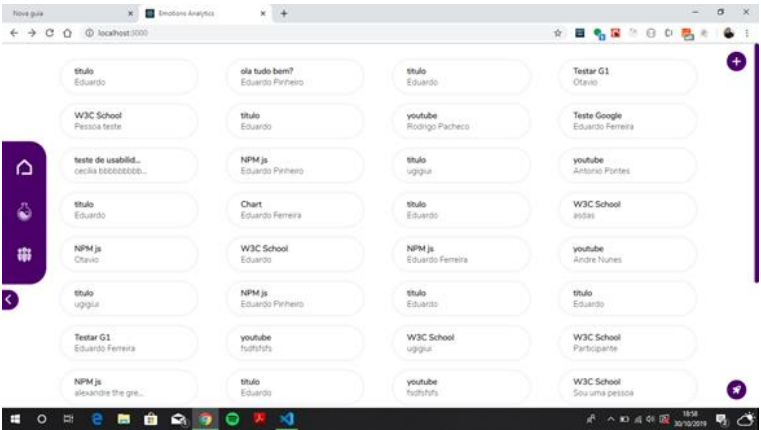
\includegraphics[width=0.7\textwidth]{1}
\end{figure}
\FloatBarrier

Ao acessar a aplicação, o usuário é direcionado para a tela inicial, conhecida como tela Home. Essa tela tem como objetivo principal exibir uma lista de todos os testes realizados até o momento. Cada teste é representado por uma célula contendo o nome do tipo de teste e o nome da pessoa que o realizou.

Na parte esquerda da tela, há botões fixos que permitem navegar entre as diferentes seções da aplicação. O botão "Home" retorna à tela inicial, o botão "Tipo de Teste" leva o usuário para a lista de tipos de teste cadastrados, e o botão "Pessoas" exibe a lista de pessoas cadastradas no sistema.

No canto direito da tela, há um grupo de botões. Os botões superiores permitem cadastrar um novo usuário e criar um novo tipo de teste. O botão inferior permite iniciar um novo teste. Esses botões estão presentes em todas as telas da aplicação, garantindo acesso rápido e fácil às funcionalidades principais do sistema.

\subsection{Tipos de teste}

Ao clicar no botão "Tipos de Teste" (ícone de recipiente de laboratório), a tela exibe as mesmas células da tela anterior, porém com um conteúdo diferente. Agora, cada célula representa um tipo de teste e exibe o título e o objetivo desse teste.

O tipo de teste é o cadastro de uma interface específica que desejamos analisar, juntamente com um objetivo previamente definido para essa análise. Por exemplo, poderíamos cadastrar um tipo de teste chamado "Teste do YouTube" com o objetivo de "analisar as reações do usuário ao descobrir o que está em alta no YouTube".

Uma vez que um tipo de teste é cadastrado, qualquer usuário pode realizar esse teste e gerar seus próprios resultados ao navegar na interface especificada. Essa funcionalidade permite a realização de análises personalizadas e a obtenção de dados relevantes sobre a experiência do usuário em diferentes interfaces.

\subsection{Pessoas}

\begin{figure}[h]
  \caption{Tela de listagem de participantes do sistema}
  \centering
  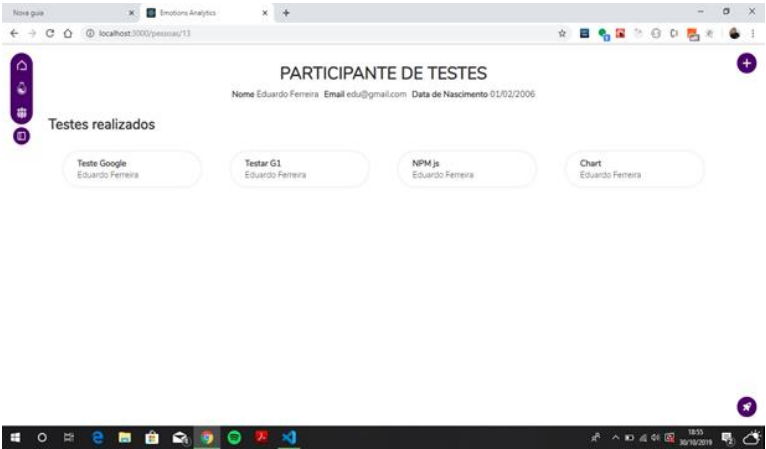
\includegraphics[width=0.7\textwidth]{2}
\end{figure}
\FloatBarrier

No canto esquerdo da tela, há o botão "Pessoas", que ao ser clicado, exibe na tela uma lista de todos os usuários cadastrados no sistema. Cada usuário é representado por uma célula contendo seu nome e e-mail.

Ao clicar em um usuário específico, a tela é atualizada para exibir informações mais detalhadas. São apresentados o nome completo do usuário, seu e-mail, data de nascimento e uma lista dos testes realizados por ele. Essas informações fornecem uma visão mais abrangente sobre cada usuário e suas atividades no sistema.

\clearpage
\subsection{Cadastro de usuário}

\begin{figure}[h]
  \caption{Tela de cadastro de usuário do sistema}
  \centering
  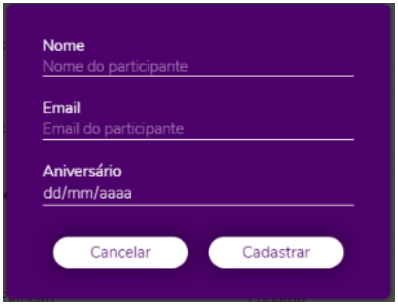
\includegraphics[width=0.7\textwidth]{3}
\end{figure}
\FloatBarrier

No canto superior direito da tela, há um conjunto de dois botões que são revelados quando clicamos no ícone "+". Um desses botões é destinado ao cadastramento de uma nova pessoa no sistema. Ao clicar nesse botão, um formulário é aberto, permitindo a coleta dos dados do usuário. O formulário contém campos para inserir o nome, e-mail e data de nascimento da pessoa. Essas informações são essenciais para o cadastro adequado do usuário no sistema.

\clearpage
\subsection{Cadastro de tipo de teste}

\begin{figure}[h]
  \caption{Tela de cadastro de tipos de teste do sistema}
  \centering
  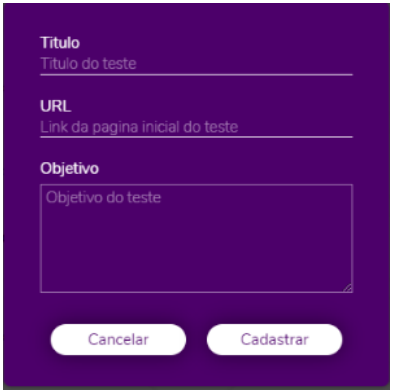
\includegraphics[width=0.7\textwidth]{4}
\end{figure}
\FloatBarrier

O outro botão presente nesse conjunto é o botão "Novo Teste". Ao clicar nele, um formulário é aberto para o cadastramento de um novo tipo de teste, conforme mencionado anteriormente. Nesse formulário, são disponibilizados campos para inserir o título do teste, a URL do site a ser analisado e o objetivo específico desse teste. Essas informações são importantes para definir o escopo e a finalidade do teste a ser realizado.

\clearpage
\subsection{Inicio do teste}

\begin{figure}[h]
  \caption{Tela de início de testes do sistema}
  \centering
  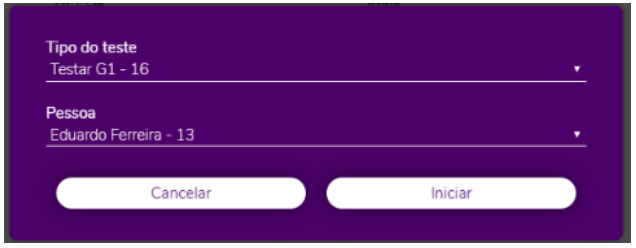
\includegraphics[width=0.7\textwidth]{5}
\end{figure}
\FloatBarrier

No canto inferior direito da tela, encontra-se o botão "Iniciar Teste" representado pelo ícone de um foguete. Ao clicar nesse botão, é iniciada a análise da interface selecionada. Antes disso, o usuário deve escolher o tipo de teste que deseja realizar e informar qual pessoa está executando o teste.

Após clicar em "Iniciar Teste", o usuário é redirecionado para a URL cadastrada no tipo de teste selecionado anteriormente. Durante o teste, a experiência é semelhante à navegação normal no site, enquanto a webcam captura o rosto da pessoa registrando suas emoções ao longo da navegação. O teste pode ser finalizado a qualquer momento por meio do botão "Finalizar" localizado no canto inferior direito da tela.

\subsection{Relatórios}

\begin{figure}[h]
  \caption{Tela de relatórios do sistema}
  \centering
  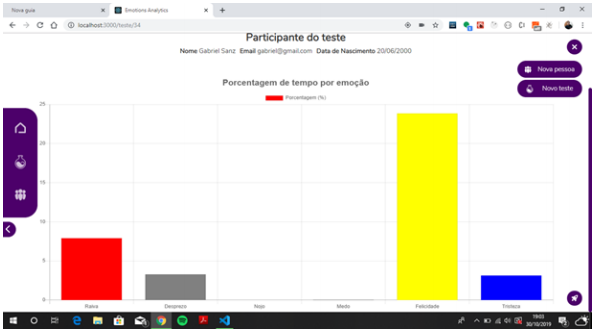
\includegraphics[width=0.7\textwidth]{6}
\end{figure}
\FloatBarrier

Ao concluir o teste, o sistema apresenta um gráfico de barras que exibe as emoções detectadas durante a navegação, representadas em porcentagem. Além disso, são fornecidas informações sobre o participante do teste. As emoções contempladas no gráfico são: raiva, desprezo, nojo, medo, felicidade e tristeza. Essas informações fornecem uma visão geral das emoções experimentadas pelo participante durante a interação com a interface analisada.

\section{Diagramas do sistema}

Os diagramas a seguir têm como objetivo fornecer uma visão mais clara e abrangente do sistema, seguindo as técnicas indicadas pelo Project Management Institute (PMI) \cite{31}. Esses diagramas são ferramentas valiosas para a representação visual das diferentes partes e interações do sistema, permitindo uma compreensão mais fácil e organizada das informações.

\subsection{Modelo de Entidade e Relacionamento do sistema}

O Modelo Entidade-Relacionamento (MER) \cite{26} é um diagrama que representa a estrutura lógica de um banco de dados, mostrando as entidades, seus atributos e os relacionamentos entre elas. Ele é útil para visualizar a organização dos dados e as conexões entre as entidades, auxiliando no projeto e implementação do sistema de gerenciamento de dados.

\begin{figure}[h]
  \caption{Diagrama de Modelo de Entidade e Relacionamento do sistema}
  \centering
  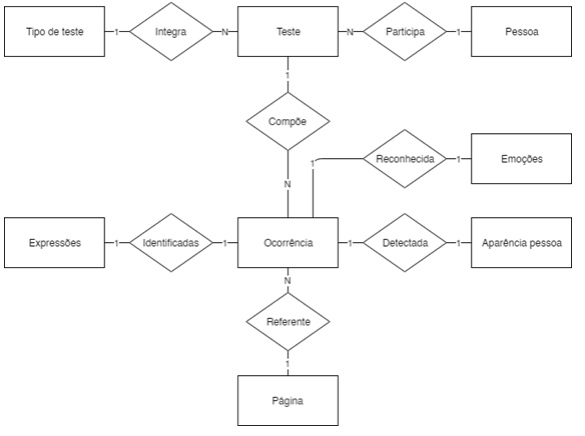
\includegraphics[width=0.7\textwidth]{7}
\end{figure}
\FloatBarrier

\clearpage
\subsection{Diagrama de casos de uso}

O Diagrama de Caso de Uso \cite{27} é uma representação visual das funcionalidades e interações do sistema a partir da perspectiva do usuário. Ele mostra os atores (usuários, sistemas externos, dispositivos, etc.) e os casos de uso, que descrevem as interações entre o sistema e os usuários. Esse diagrama é útil para entender os requisitos e as principais funcionalidades do sistema.

\begin{figure}[h]
  \caption{Diagrama de casos de uso do sistema}
  \centering
  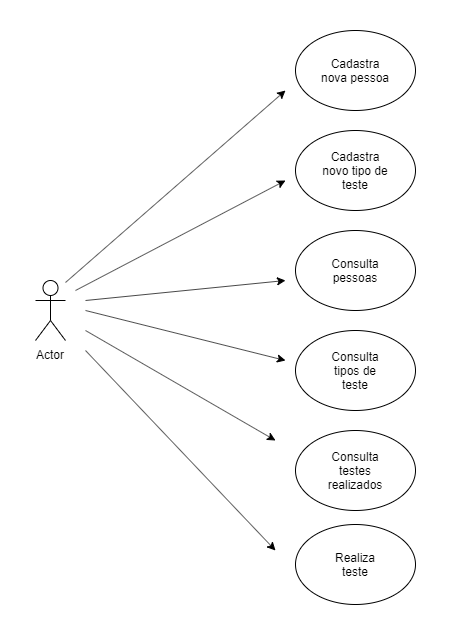
\includegraphics[width=0.7\textwidth]{8}
\end{figure}
\FloatBarrier

\clearpage
\subsection{Diagrama de classes}

O diagrama de classes \cite{27} é uma representação visual das classes, seus atributos e métodos, bem como os relacionamentos entre as classes. Ele fornece uma visão abrangente da estrutura do sistema, mostrando como as classes interagem entre si e quais são suas propriedades. Esse diagrama é fundamental para o design orientado a objetos, auxiliando no desenvolvimento e na compreensão do sistema de software.

\begin{figure}[h]
  \caption{Diagrama de classes do sistema}
  \centering
  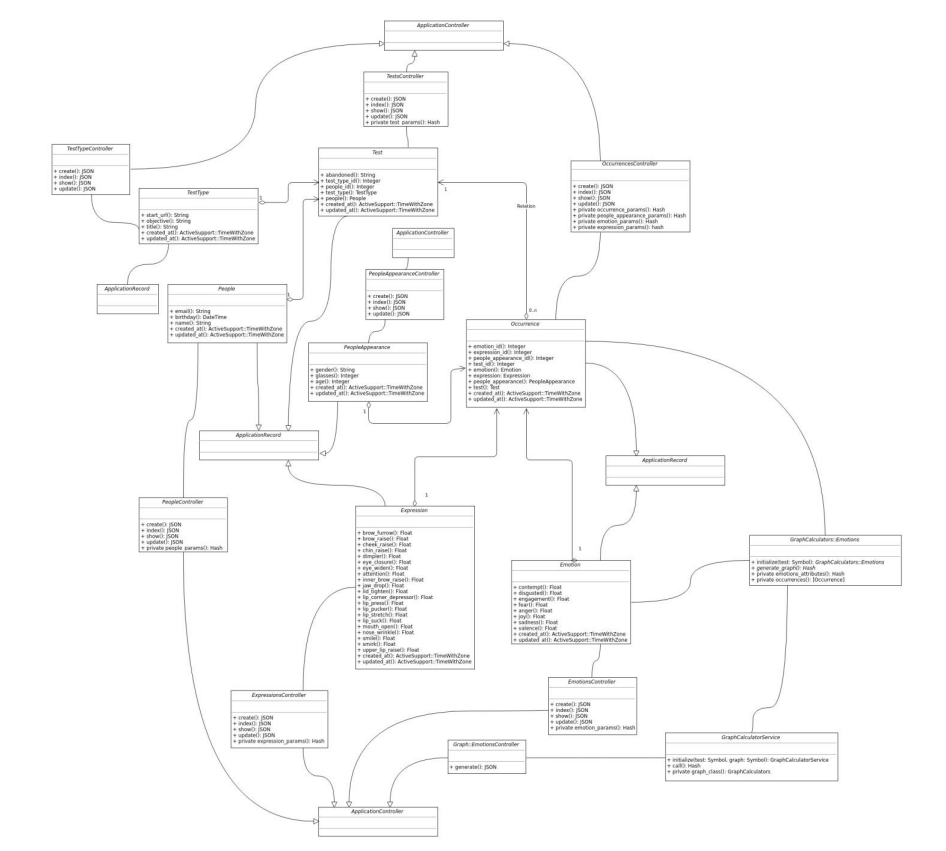
\includegraphics[width=0.7\textwidth]{9}
\end{figure}
\FloatBarrier

\clearpage
\subsection{Diagramas de sequência}

O Diagrama de Sequência \cite{28} é utilizado para representar a interação entre os objetos do sistema ao longo do tempo. Ele mostra a ordem das mensagens trocadas entre os objetos e como eles colaboram para realizar uma determinada funcionalidade. Esse diagrama é útil para entender o fluxo de execução e a comunicação entre os objetos do sistema.

\begin{figure}[h]
  \caption{Diagrama de sequência de criação, edição, leitura e deleção do endpoint TestType do sistema}
  \centering
  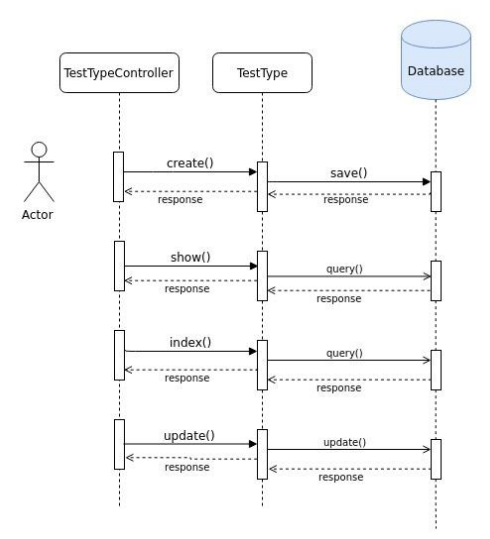
\includegraphics[width=0.7\textwidth]{10}
\end{figure}
\FloatBarrier

\begin{figure}[h]
  \caption{Diagrama de sequência de criação, edição, leitura e deleção do endpoint Tests do sistema}
  \centering
  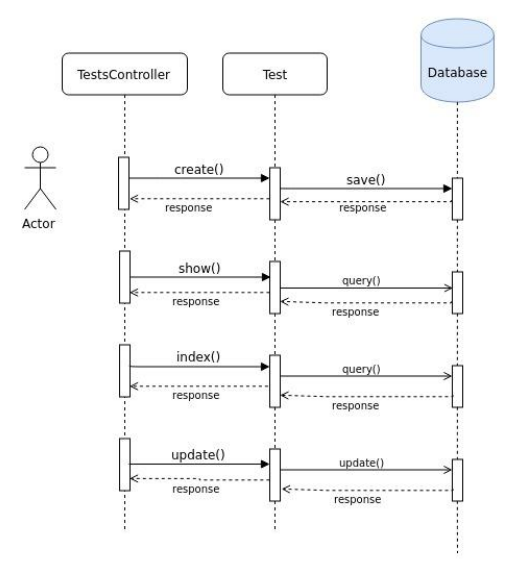
\includegraphics[width=0.7\textwidth]{11}
\end{figure}
\FloatBarrier

\begin{figure}[h]
  \caption{Diagrama de sequência de criação, edição, leitura e deleção do endpoint People do sistema}
  \centering
  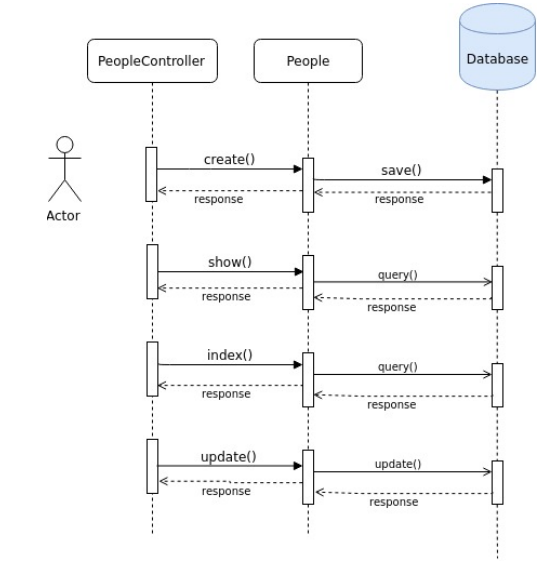
\includegraphics[width=0.7\textwidth]{12}
\end{figure}
\FloatBarrier

\begin{figure}[h]
  \caption{Diagrama de sequência de criação, edição, leitura e deleção do endpoint PeopleAppearence do sistema}
  \centering
  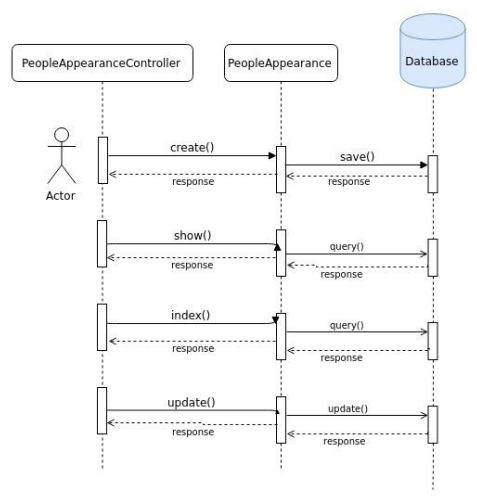
\includegraphics[width=0.7\textwidth]{13}
\end{figure}
\FloatBarrier

\begin{figure}[h]
  \caption{Diagrama de sequência de criação, edição, leitura e deleção do endpoint Expressions do sistema}
  \centering
  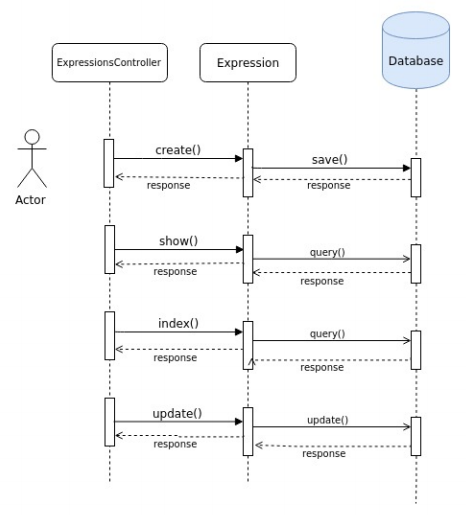
\includegraphics[width=0.7\textwidth]{14}
\end{figure}
\FloatBarrier

\begin{figure}[h]
  \caption{Diagrama de sequência de criação, edição, leitura e deleção do endpoint Emotions do sistema}
  \centering
  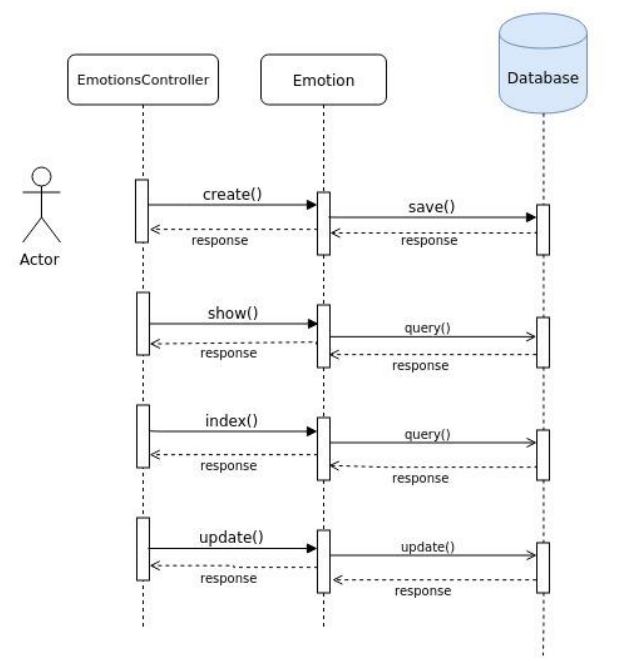
\includegraphics[width=0.7\textwidth]{15}
\end{figure}
\FloatBarrier

\begin{figure}[h]
  \caption{Diagrama de sequência de criação, edição, leitura e deleção do endpoint Occurences do sistema}
  \centering
  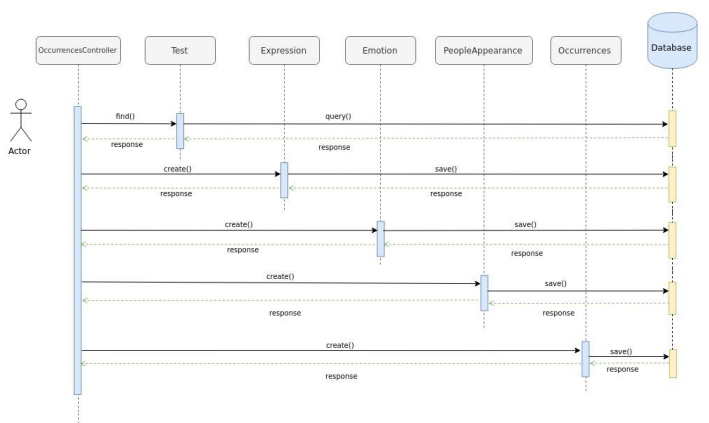
\includegraphics[width=0.7\textwidth]{16}
\end{figure}
\FloatBarrier

\subsection{Diagramas de máquina de estado}

O diagrama de máquina de estados \cite{30} é uma representação visual que descreve o comportamento de um objeto ou sistema em diferentes estados e as transições entre esses estados. Ele mostra como um objeto ou sistema responde a eventos e como seu estado muda ao longo do tempo. O diagrama de máquina de estados é composto por estados, transições, eventos e ações, e é útil para modelar o comportamento complexo de sistemas que possuem diferentes estados e interações entre eles. Ele permite uma compreensão clara do fluxo de controle e das possíveis sequências de eventos que podem ocorrer em um sistema.

\begin{figure}[h]
  \caption{Diagrama de maquina de estado para cadastro de pessoa no sistema}
  \centering
  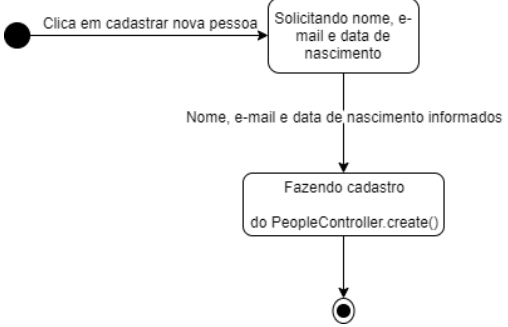
\includegraphics[width=0.7\textwidth]{17}
\end{figure}
\FloatBarrier

\begin{figure}[h]
  \caption{Diagrama de maquina de estado para cadastro de tipo de teste no sistema}
  \centering
  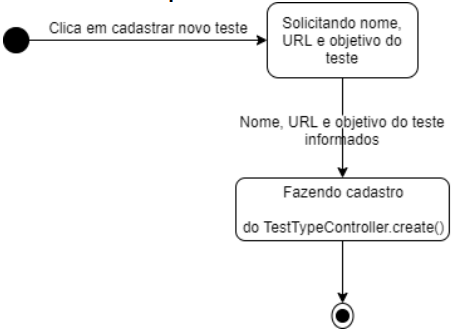
\includegraphics[width=0.7\textwidth]{18}
\end{figure}
\FloatBarrier

\begin{figure}[h]
  \caption{Diagrama de maquina de estado para consulta de pessoa no sistema}
  \centering
  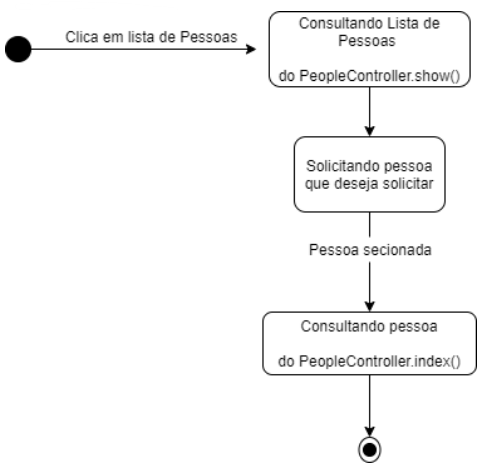
\includegraphics[width=0.7\textwidth]{19}
\end{figure}
\FloatBarrier

\begin{figure}[h]
  \caption{Diagrama de maquina de estado para consulta de tipos de teste no sistema}
  \centering
  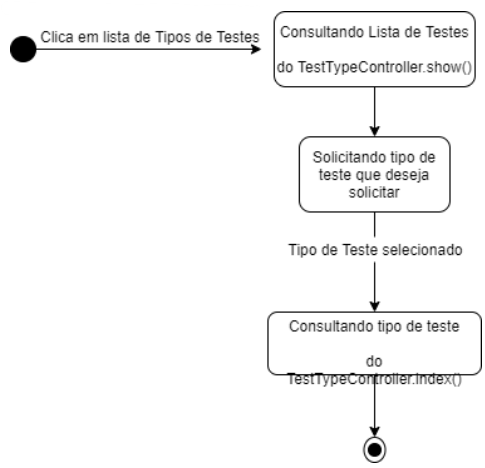
\includegraphics[width=0.7\textwidth]{20}
\end{figure}
\FloatBarrier

\begin{figure}[h]
  \caption{Diagrama de maquina de estado para realizar teste no sistema}
  \centering
  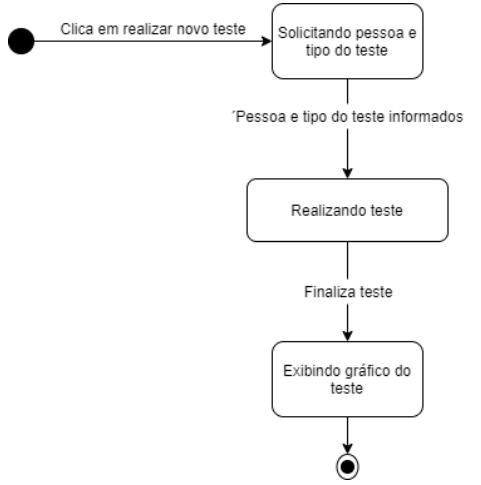
\includegraphics[width=0.7\textwidth]{21}
\end{figure}
\FloatBarrier

\begin{figure}[h]
  \caption{Diagrama de maquina de estado para consulta de teste no sistema}
  \centering
  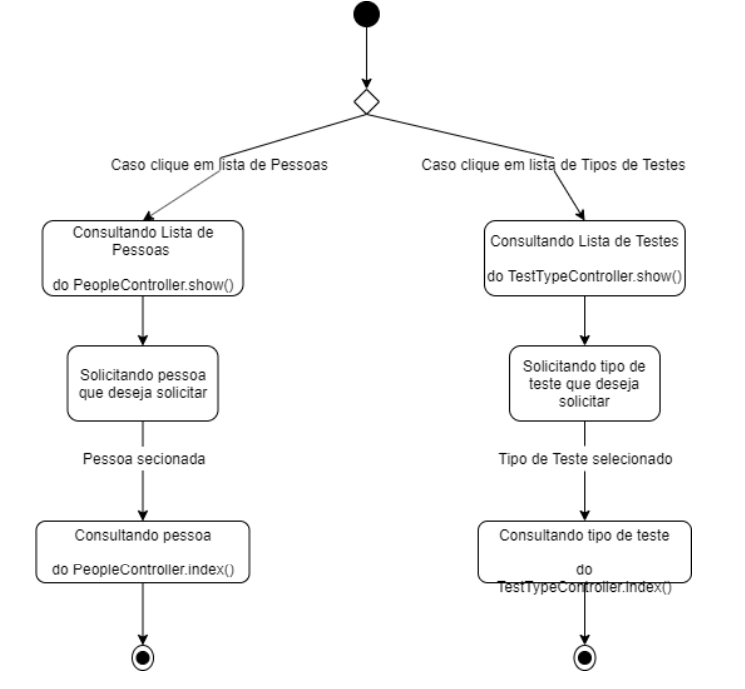
\includegraphics[width=0.7\textwidth]{22}
\end{figure}
\FloatBarrier
